\documentclass[titlepage,a4paper,12pt]{ltjsreport}

\usepackage{luatexja}
\usepackage{amsmath,amsfonts}
\usepackage{amsthm}
\usepackage{bm}
\usepackage[dvipdfmx]{graphicx}
\usepackage{color}
\usepackage{here}
\usepackage{caption}
\usepackage{url}
\usepackage{listings}
\usepackage{abstract}
\usepackage{multicol}
\usepackage{geometry}
\usepackage{here}

\lstset{
    basicstyle={\ttfamily},
    identifierstyle={\small},
    commentstyle={\small},
    keywordstyle={\small\bfseries},
    ndkeywordstyle={\small},
    stringstyle={\small\ttfamily},
    frame={tb},
    breaklines=true,
    columns=fixed,
    basewidth=0.465em,
    numbers=left,
    numberstyle={\scriptsize},
    lineskip=-0.5ex
}


\begin{document}

\leftline{課題1 要求記述}
\rightline{256E0143
三留 慎太郎}

\begin{enumerate}
    \item 概要 \mbox{}\\
    $n$個の実数の集合の平均$x_avg$と標準偏差$\sigma$を計算する。\\


    \item 詳細\mbox{}\\
    平均$x_{avg}$と標準偏差$\sigma$は以下の式で求められる。
    \[x_{avg} = \frac{\sum^{n}_{i=1}x_i}{n}\]
    \[\sigma = \sqrt{\frac{\sum^{n}_{i=1}(x_i - x_{avg})^2}{n-1}}\]
    
    ここで$n$は与えられる実数の数、$x_i$は$i$個目の実数の値を表す。\\
    また、与えられる$n$個の実数は、双方向リンクリストを用いて操作する。


    \item 入力\mbox{}\\
    
    \begin{itemize}
        \item 実数値の入力:ファイル入力
        \item 実数値入力ファイル:ファイル例の図\ref{value_example}のように、ファイルの中身は実数を改行で区切ったもの。
        
        \begin{figure}[h]
            \centering
            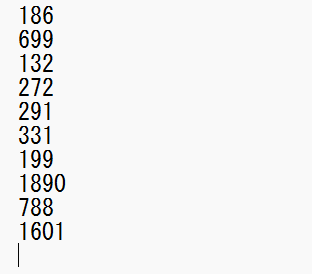
\includegraphics[width=0.4\textwidth]{../picture/value_example.png}
            \caption{実数入力ファイル例}
            \label{value_example}
        \end{figure}
        
        \item 実行時の入力:コマンドラインに以下の形式で入力
         java プログラム名 実数値入力ファイル名
        \item 実行時入力例:java Program1 input1.txt

    \end{itemize}


    \item 出力\mbox{}\\
    \begin{itemize}
        \item 出力方法:コマンドライン出力
        \item 出力する値:平均値$x_{avg}$、標準偏差$\sigma$
        \item 精度:平均値、標準偏差共に小数点第2位までを小数点以下第3位を四捨五入したものとする。
        \item 出力例:図\ref{out_example}のようにそれぞれ改行して表示する。
        
        \begin{figure}[h]
            \centering
            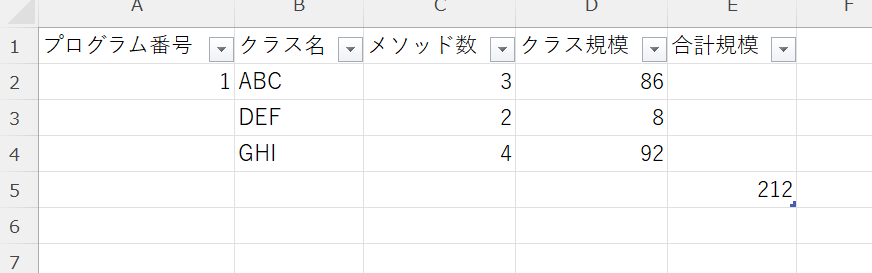
\includegraphics[width=0.4\textwidth]{../picture/out_example.png}
            \caption{出力例}
            \label{out_example}
        \end{figure}

    \end{itemize}

    \item 実行方法\mbox{}\\
    コマンドラインに
     java Program1 input1.txt
    と入力して実行する。
    \item テスト\mbox{}\\
    表\ref{test_data}のデータを用いて表\ref{test}のテストを行う。
    \begin{table}[h]
        \centering
        \caption{Testdata}
        \label{test_data}
        \begin{tabular}{|c|c|} \hline
            Column1 & Column2 \\ \hline
            Estimate Proxy Size & Development Hours \\ \hline
            160   & 15.0 \\ \hline
            591   & 69.9 \\ \hline
            114   & 6.5 \\ \hline
            229   & 22.4 \\ \hline
            230   & 28.4 \\ \hline
            270   & 65.9 \\ \hline
            128   & 19.4 \\ \hline
            1657  & 198.7 \\ \hline
            624   & 38.8 \\ \hline
            1503  & 138.2 \\ \hline
        \end{tabular}
    \end{table}

    \begin{table}[h]
        \centering
        \caption{Test}
        \label{test}
        \begin{tabular}{|c|c|c|} \hline
            入力 & \multicolumn{2}{|c|}{期待値} \\ \hline
            & 平均 & 標準偏差 \\ \hline
            表1:Column1 & 550.6 & 572.03 \\ \hline
            表1:Column2 & 60.32 & 62.26 \\ \hline
        \end{tabular}
    \end{table}
    
     

\end{enumerate}



\end{document}